\chapter{Was Quantenphänomene über den verborgenen Aufbau sagen}
\label{ch:shadow-quantum}
\begin{bild}{Nicht nur die Anzahl der Kugeln zählt}
Zwei Kästen können dieselben möglichen Messergebnisse enthalten und doch verschieden reagieren, wenn wir zuerst an einer anderen Stelle messen oder zwei Teile zusammenführen. Die Quantenphänomene sagen uns deshalb vor allem etwas über die Regeln des Zusammensetzens, über relative Phasen und über erlaubte Eingriffe. Genau diese Daten verliert ein einfacher Schatten leicht.
\end{bild}

\section{Interferenz verlangt eine Information vor den Wahrscheinlichkeiten}
Für zwei Alternativen mit Amplituden $a$ und $b$ lautet die Born-Regel
\[
 P_{ab}=|a+b|^2=|a|^2+|b|^2+2\Re(a\bar b).
\]
Der letzte Term kann verstärken oder auslöschen. Wer ausschließlich die beiden Einzelwahrscheinlichkeiten aufbewahrt, kann ihn nicht rekonstruieren. Das erklärt im Kleinen, warum die behaltenen Register und Echoexperimente der früheren Kapitel mehr verraten als der erste sichtbare Markovschritt.

Für drei unter denselben idealen Bedingungen zusammengesetzte Alternativen gilt exakt
\begin{equation}
 I_3=P_{abc}-P_{ab}-P_{ac}-P_{bc}+P_a+P_b+P_c=0.
\end{equation}
Dies ist die algebraische Folge der quadratischen Born-Regel, hier für beliebige komplexe $a,b,c$ symbolisch kontrolliert. Dreispaltexperimente begrenzen Abweichungen von dieser Vorhersage; die reale Änderung der Randbedingungen beim Öffnen eines Spalts muss in der Auswertung berücksichtigt werden. Eine endliche Fehlerschranke beweist keine absolut exakte Null in der Natur. \src{F08}

\textbf{Constraint für den Universalraum:} Ein Modell muss Phasen vor der Wahrscheinlichkeitsbildung tragen, ihre Zusammensetzung erklären und die beobachtete Interferenzordnung reproduzieren. Es reicht nicht, die Born-Regel nachträglich als Ausleseformel einzusetzen und damit ihre Herkunft als gelöst zu bezeichnen.

\section{Der vorhandene Baukasten enthält bereits Kontextualität}
Die 15 Zwei-Qubit-Pauli-Kontexte der Synthese enthalten das folgende Mermin--Peres-Quadrat. Hier bedeutet $XI=X\otimes I$ und entsprechend für die anderen Einträge:
\begin{figure}[H]\centering
\begin{tikzpicture}[x=2.25cm,y=1.05cm]
\foreach \x/\y/\t in {0/2/XI,1/2/IX,2/2/XX,0/1/IZ,1/1/ZI,2/1/ZZ,0/0/XZ,1/0/ZX,2/0/YY}
 {\node[box,minimum width=18mm,minimum height=8mm] at (\x,\y) {$\t$};}
\foreach \y in {0,1,2}{\node[text=teal,font=\sffamily] at (3.1,\y) {Produkt $+I$};}
\node[text=teal] at (0,-.9) {$+I$};\node[text=teal] at (1,-.9) {$+I$};\node[text=amber] at (2,-.9) {$-I$};
\node[font=\sffamily\small,text=slate] at (1.1,-1.6) {Spaltenprodukte: genau ein Minuszeichen};
\end{tikzpicture}
\caption{Jede Zeile und jede Spalte ist gemeinsam messbar. Alle Zeilenprodukte sind positiv, aber das letzte Spaltenprodukt ist negativ. Diese sechs Kontexte gehören zum bereits verwendeten Pauli-System.}
\end{figure}

Angenommen, jede der neun Größen hätte vor der Messung einen festen, vom Kontext unabhängigen Wert $\pm1$, und diese Werte respektierten die Produktregel für gemeinsam messbare Größen. Multipliziert man alle sechs Kontextgleichungen, erscheint jeder Einzelwert zweimal: links muss $+1$ stehen. Die rechten Seiten ergeben aber $-1$. Das ist ein Widerspruch. Die neue Gegenrechnung prüft alle Operatorprodukte und zusätzlich sämtliche $2^9=512$ möglichen Wertzuweisungen. Keine erfüllt alle Bedingungen. \src{F09; eigener Nachbau}

Das Ergebnis ist \emph{zustandsunabhängig}; die Identitäten gelten als Operatorgleichungen. Es sagt nicht, dass jede klassische Simulation unmöglich sei. Der eingeschränkte Clifford-/Stabilizer-Baukasten kann effizient simulierbar sein und trotzdem diese naive, kontextunabhängige Wertvorstellung ausschließen. Auch der passive 60-Zustands-Prozess ist kein Gegenbeweis gegen Kontextualität: Er verfolgt nicht automatisch alle Eingriffe mit einer einheitlichen vorab festgelegten Wertzuweisung.

\textbf{Folgerung:} Die reichere Struktur muss mindestens Messkontexte und ihre gemeinsamen Observablen bewahren. Die bloße Liste möglicher Ergebnisse, ihre Anzahl 60 oder eine stationäre Verteilung bewahrt zu wenig. Damit erhält die im Buch geforderte Algebra der erlaubten Operationen einen sehr konkreten Grund.

\section{Verschränkung legt die Zusammensetzung fest}
Für zwei räumlich getrennte Messstellen hat die CHSH-Kombination
\[
 S=\langle A_0B_0\rangle+\langle A_0B_1\rangle
 +\langle A_1B_0\rangle-\langle A_1B_1\rangle
\]
in einem lokalen Modell mit unabhängiger Wahl der Einstellungen die Grenze $|S|\leq2$. Quantenmechanik erreicht $2\sqrt2$. Mit $A_0=Z$, $A_1=X$ und $B_{0,1}=(Z\pm X)/\sqrt2$ ist der zugehörige Operator $\sqrt2(ZZ+XX)$; seine Eigenwerte sind $-2\sqrt2,0,0,2\sqrt2$. Beides wurde hier exakt nachgerechnet. Bell-Experimente prüfen solche Unterschiede unter sorgfältig formulierten Bedingungen. \src{F07}

Kein nutzbares Überlichtsignal folgt aus einer Verletzung. Umgekehrt reicht die Forderung \glqq kein Signal\grqq{} allein nicht zur Quantenmechanik: Allgemeine nichtsignalisierende Korrelationen können den algebraischen Wert 4 erreichen. Die gesuchte Struktur muss daher mehr auswählen als bloße Nichtsignalisierung. Sie muss die spezielle quantenmechanische Menge gemeinsam möglicher Korrelationen reproduzieren.

Für die TFPT-Zellen bedeutet dies: Die lokale Dimension 4 und ein singulärer Vierträgerzustand liefern geeignete endliche Zutaten. Dass entfernte physikalische Zellen tatsächlich die richtigen lokalen Messalgebren, Einstellungen und Korrelationen besitzen, bleibt ein zusätzlicher dynamischer und räumlicher Nachweis. Das algebraische Beispiel ist noch kein Bell-Experiment an TFPT-Materie.

\section{Gleiche Energien können verschiedene Welten beschreiben}
Wähle bei festgehaltenen Labor-Teilsystemen
\[
 H_0=Z\otimes I+2I\otimes Z,
 \quad U=\mathrm{CNOT}(H_{\mathrm{Had}}\otimes I),
 \quad H_1=UH_0U^\dagger.
\]
Beide Hamiltonoperatoren haben exakt die Energien $-3,-1,1,3$. Der Grundzustand von $H_0$ ist ein Produktzustand, der von $H_1$ ein Bell-Zustand. Die Reinheit $\Tr\rho_A^2$ eines lokalen Teils beträgt entsprechend 1 beziehungsweise $1/2$.

\begin{figure}[H]\centering
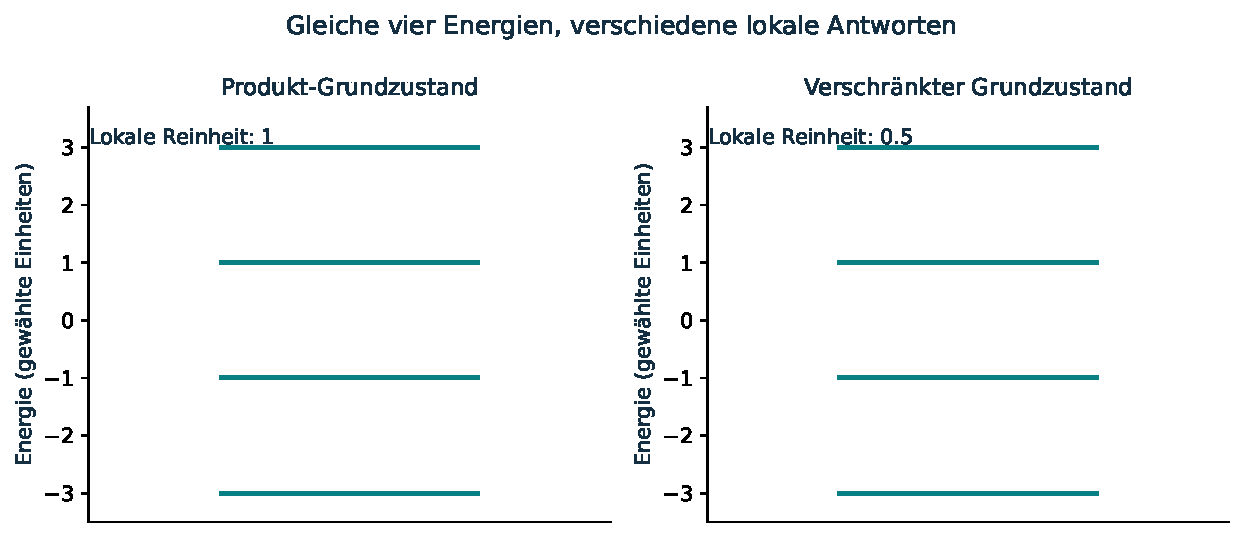
\includegraphics[width=\linewidth]{figures/shadow_isospectral.pdf}
\caption{Eine Liste von Energien erkennt die lokale Verschränkung nicht. Hier bleiben die Laboralgebren fest; würden auch alle Observablen mittransformiert, wäre es nur ein Darstellungswechsel.}
\end{figure}

Diese Gegenprobe verdichtet die Spektralfrage des RH-Zweigs: Selbst eine exakte Liste richtiger Eigenwerte bestimmt die physikalische Lokalität und die messbaren Antworten noch nicht. Dazu gehören Eigenvektoren relativ zu einer beobachtbaren Algebra und gemischte Korrelationsfunktionen. Die Zuordnung eines Tensorprodukts ist selbst durch die verfügbaren Observablen bestimmt. \src{E10; eigene Rechnung}

\section{Was komplexe Zahlen verraten und was offenbleibt}
Die komplexe Vierdimensionalität ist für den bestehenden Pauli-/Spinorbaukasten passend. Eine direkte Ableitung der komplexen Zahlen aus einem einzelnen Quantenphänomen wäre trotzdem zu stark. Renou und Mitautoren untersuchen Quantennetzwerke, in denen die übliche reale und komplexe Theorie unter einer bestimmten Unabhängigkeits- und Kompositionsannahme verschiedene Vorhersagen machen. \src{F10}

Eine Arbeit von Hoffreumon und Woods aus März 2026 unterscheidet operative Unabhängigkeit von einer faktorisierenden mathematischen Beschreibung und formuliert einen realen Simulationsrahmen. Ein Kommentar vom April diskutiert wiederum die Verträglichkeit vorgeschlagener Prinzipien mit fermionischer Informationstheorie. Diese neuen Arbeiten werden hier als fachliche Debatte eingeordnet, nicht als endgültige Entscheidung über die Natur der Zahlen. \src{F11, F12}

Die belastbare Verdichtung lautet: \emph{Experimentell bedeutsam ist das gemeinsame Paket aus Zustandsraum, erlaubten Operationen, Zusammensetzung und Unabhängigkeit.} Ein Wechsel von $\C$ nach $\R$ bei gleichzeitig veränderter Zusammensetzungsregel ist kein bloßer Austausch eines Symbols. Unsere Universalraum-Hypothese muss genau dieses Paket auswählen.

\section{Messung, Zeitpfeil und Statistik}
Die bisherigen Registerbeispiele erklären, wie ein global kohärenter Ablauf nach eingeschränktem Zugriff wie ein irreversibler Prozess aussehen kann. Sie liefern noch keine eindeutige Lösung des Messproblems: Insbesondere folgt aus einer diagonalen reduzierten Dichtematrix allein keine Auswahl eines einzelnen Ereignisses. Eine zusätzliche Kollapsdynamik müsste messbare Abweichungen angeben; eine unitäre Beschreibung müsste die Rolle stabiler Aufzeichnungen und der verwendeten Wahrscheinlichkeiten klären.

Ebenso ist eine nichttriviale Phase nicht automatisch Wärmeproduktion. Eine ideale unitäre Phasenoperation ist reversibel. Thermodynamische Löschkosten betreffen konkrete Ressourcen und Zugriffsmöglichkeiten; bei Quantenspeicher kann sogar die bedingte Entropie negativ sein, ohne dass die globale Entropiebilanz verletzt wird. \src{F13}

Auch Bosonen und Fermionen entstehen nicht allein dadurch, dass eine Wurzelsumme fehlt. Die Austauschstatistik verlangt Mehrteilchenzustände und deren Austauschoperationen; ein Spin-Statistik-Satz verwendet weitere Voraussetzungen wie relativistische Lokalität und Positivität. Die \glqq harte Hülle\grqq{} aus dem Ursprungsteil bleibt daher eine klar benannte zusätzliche Regel. Sie gewinnt durch das Wort Quantenphänomen keine neue Herleitung.
